


\begin{frame}{Local Input Space Histograms \sof{1}{3}}

\vspace{1.5em}
\justifying
Prototype-based clustering methods like the {\bf growing neural gas} (GNG) can
suffer from a lack of detail in their input space representation. To amend their
descriptive power we introduced the novel concept of {\bf local input space 
histograms} (LISH) that capture statistical information on the input space lying
between neighboring prototypes~\cite{Kerdels2014a}.

\vspace{1.5em}

\twocol{0.41}{
\justifying
In a regular GNG neighboring prototypes are connected by an edge. We added a 
small histogram to each edge to {\bf capture information on the positions of 
input samples} relative to the respective best and second best matching 
prototypes. 

}{0.5}{
\vspace{-2em}
\begin{figure}
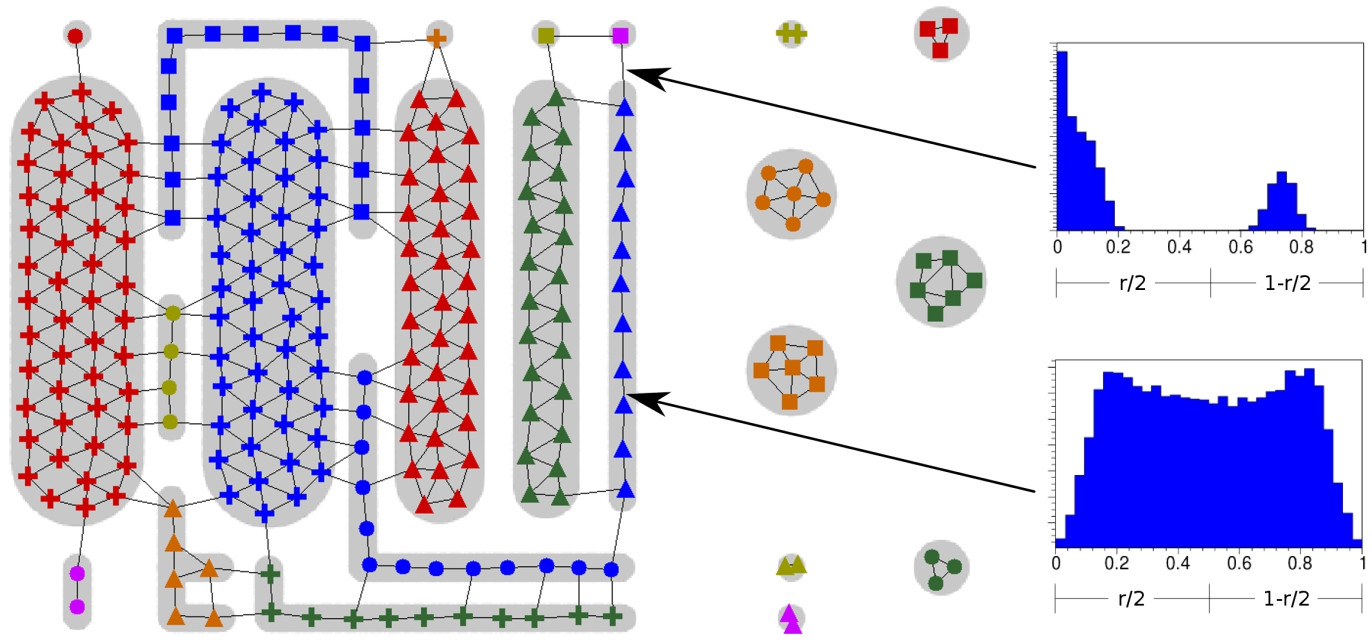
\includegraphics[width=\linewidth]{lish/lish.jpg}

\vspace{-1em}
\caption{\scriptsize Clustering of an inhomogeneous input space (gray areas) 
with a GNG network of 250 units resulting in 23 clusters (marked by shapes and 
colors of the units). Histograms of two edges are shown on the 
right~\cite{Kerdels2014a}.}
\end{figure}
}

\vspace{1em}
We were able to demonstrate that this additional information can be utilized to,
e.g., {\bf improve clustering} results for challenging, inhomogeneous input 
spaces.

\begin{center}
\rule{2cm}{0.4pt}\\[0.5em]
\end{center}

\fc{Kerdels2014a}{publications/2014-01/2014-01}

\end{frame}



\begin{frame}{Local Input Space Histograms \sof{2}{3}}

\twocol{0.4}{
\vspace{-4em}
\begin{figure}
\adjincludegraphics[width=1.\linewidth,valign=t]{lish/force-based.jpg}
\vspace{-1.25em}
\caption{\scriptsize Foo~\cite{Kerdels2015}.}
\adjincludegraphics[width=1.\linewidth,valign=b]{lish/hierarchical.jpg}
\vspace{-1.5em}
\caption{\scriptsize Bar~\cite{Kerdels2015}.}
\end{figure}
}{0.55}{
\justifying
Foo

\vspace{1em}
The analysis was featured on the title page of ``Informatik 
Spektrum''~\cite{Kerdels2015c}, the main organ of the German Informatics 
Society~(GI).

}

\begin{center}
\rule{2cm}{0.4pt}\\[0.5em]
\end{center}

\fc{Kerdels2015}{publications/2015-02/2015-02}\\[1em]
\fc{Kerdels2015c}{publications/2015-03/2015-03}

\end{frame}


\begin{frame}{Local Input Space Histograms \sof{3}{3}}

%\vspace{1em}
\justifying
Foo


\vspace{2em}



\begin{center}
\rule{2cm}{0.4pt}\\[0.5em]
\end{center}

\fc{Kerdels2016b}{publications/2016-02/2016-02}

\end{frame}


